\documentclass[conference]{IEEEtran}
\usepackage[utf8]{inputenc}
\usepackage[T1]{fontenc}
\usepackage[spanish,es-tabla,es-nodecimaldot]{babel}
\usepackage{graphicx,booktabs,amsmath,cite,url,array}
\usepackage[hidelinks]{hyperref}

\begin{document}

\title{Hogar, colegio y municipio en Saber~11 de 2025:\\ agrupación, árboles de decisión y bandits contextuales}

\author{\IEEEauthorblockN{Camilo Alejandro Lagos Malaver}
\IEEEauthorblockA{Introducción a los Sistemas Inteligentes, 2026-2\\
Depto. de Ingeniería de Sistemas e Industrial\\
Universidad Nacional de Colombia, Bogotá\\
clagosm@unal.edu.co}
\and
\IEEEauthorblockN{Luis Gabriel Peraza Muñoz}
\IEEEauthorblockA{Introducción a los Sistemas Inteligentes, 2026-2\\
Depto. de Ingeniería de Sistemas e Industrial\\
Universidad Nacional de Colombia, Bogotá\\
lperazam@unal.edu.co}}

\maketitle

\begin{abstract}
Aplicamos tres técnicas de aprendizaje maquinal a \emph{todos} los resultados del examen Saber~11 de 2025 (microdatos de DataIcfes, 561.049 estudiantes de colegio de los dos periodos), cruzados con la pobreza multidimensional municipal del DANE y con indicadores agregados de cada colegio. Un árbol J48 (Weka) predice si un estudiante queda sobre la mediana con 70,7\,\% de exactitud (AUC 0,77) frente a 50,2\,\% de la línea base; las nuevas variables y los cruces suben la exactitud dos puntos frente al conjunto usado con los datos de 2022. K-means (Weka) aplicado a 9.692 colegios separa cuatro tipos con 85 puntos de diferencia entre el más rico y el rural más pobre, mientras que a nivel de estudiante los grupos resultan inestables. Un bandit contextual LinUCB, simulado sobre datos fijos, aprende a identificar el área más débil de cada estudiante y reduce el arrepentimiento 14,6\,\% frente al azar. El hallazgo central es que el contexto del colegio pesa más que el del hogar: un estudiante de estrato~1 en un colegio de nivel socioeconómico alto obtiene en promedio 91 puntos más que uno de estrato~1 en un colegio de nivel bajo.
\end{abstract}

\begin{IEEEkeywords}
Saber 11, DataIcfes, K-means, J48, bandit contextual, LinUCB, Weka, pobreza multidimensional.
\end{IEEEkeywords}

\section{Introducción}
El examen Saber~11 del ICFES evalúa matemáticas, lectura crítica, sociales y ciudadanas, ciencias naturales e inglés al terminar la educación media. Cada registro trae además un cuestionario socioeconómico y datos del colegio, lo que permite estudiar la relación entre el contexto y el desempeño con técnicas de los tres paradigmas del curso.

Una primera versión de este trabajo usó los datos abiertos de 2022~\cite{icfes22} (530.815 estudiantes de calendario~A, 18 variables). Esta versión usa el año más reciente disponible, 2025, con los microdatos completos de DataIcfes: más estudiantes, 48 variables y dos cruces con otras fuentes. Planteamos cuatro preguntas: (P1) ¿qué tipos de estudiantes y de colegios existen y cómo les va? (P2) ¿qué variables predicen si un estudiante queda en la mitad superior, y cuánto aportan las nuevas variables y los cruces? (P3) ¿puede un tutor virtual identificar, usando solo el perfil, el área en que cada estudiante está más rezagado? (P4) ¿qué cambió frente a 2022?

\section{Datos, cruces y preprocesamiento}
\textbf{Fuente principal.} Microdatos de Saber~11 de los periodos 20251 y 20252 descargados de DataIcfes (acceso con registro)~\cite{dataicfes}: 20251 trae 85.678 filas y 85 columnas, y 20252, 576.213 filas y 92 columnas. Las 7 columnas que solo trae 20252 son \texttt{fami\_numhermanos}, \texttt{estu\_comunidadcampesina}, \texttt{estu\_numhijos}, \texttt{estu\_horastrabnoremu}, \texttt{fami\_posicionhermanos}, \texttt{estu\_tiempocasaacole} y \texttt{estu\_desplazacolegio}; la unión de ambos periodos tiene 92 columnas (en 20251 esas siete quedan como faltantes). Antes de deduplicar hay 661.891 inscritos; al eliminar duplicados por \texttt{estu\_consecutivo} quedan 661.889 (solo 2 duplicados). Nos quedamos con los 569.174 estudiantes de colegio (los individuales no traen datos de colegio) y descartamos 8.125 sin alguno de los cinco puntajes: trabajamos con \textbf{561.049 estudiantes} (21.675 del periodo 20251 y 539.374 del 20252), sin muestreo.

\textbf{Cruce 1: municipio.} Unimos cada estudiante con el índice de pobreza multidimensional (IPM) municipal de fuente censal 2018 del DANE~\cite{dane}, por el código DANE del municipio del colegio. El IPM es un indicador \emph{municipal} (del municipio donde está el colegio), no del estudiante ni de su hogar. El cruce cubre al 99,98\,\% de los estudiantes. Además del IPM total usamos el IPM rural y dos privaciones (bajo logro educativo y trabajo informal), y discretizamos el IPM en cuatro niveles ($<$20, 20--35, 35--50, $>$50). Esto impone una limitación ecológica: a partir del IPM municipal no se puede inferir la pobreza del hogar de un estudiante.

\textbf{Cruce 2: colegio.} Con el código DANE del establecimiento agregamos, \emph{sin usar puntajes} para no filtrar la respuesta, el número de evaluados, el porcentaje con computador en casa, el porcentaje de estrato~1 y el de madres profesionales. Con estos indicadores y el IPM armamos también una base de \textbf{9.692 colegios} con al menos 10 evaluados.

\textbf{Atributos.} Para clasificar usamos 48 atributos nominales: los 18 de la versión 2022 (\texttt{estu\_genero}, edad al examen, estrato, educación de los padres, bienes del hogar, naturaleza, área, jornada, bilingüismo, carácter, \texttt{cole\_genero} y departamento del colegio) más 27 nuevos de 2025 (nivel socioeconómico del colegio calculado por el ICFES, libros en casa, horas de trabajo, horas de lectura e internet, alimentación, ocupación de los padres, etnia, comunidad campesina, tiempo y medio de transporte al colegio, entre otros) y 3 de los cruces. Los faltantes se dejaron como \texttt{?}; el 7,5\,\% no respondió el cuestionario del hogar.

\textbf{Clase.} \emph{Alto} si el puntaje global supera la mediana de 2025 (254 puntos); quedan 279.656 Alto y 281.393 Bajo.

\textbf{Herramientas.} Preprocesamiento en Python (pandas) con exportación a ARFF; K-means y J48 en Weka 3.8.6~\cite{weka} por línea de comandos con 6~GB de memoria; el bandit en Python con NumPy. El código y los resultados están en el repositorio público del proyecto~\cite{repo}; los microdatos no se incluyen por su licencia de acceso restringido.

\section{Técnica 1: agrupación con K-means}
\subsection{Método}
Usamos \texttt{SimpleKMeans} de Weka en dos niveles. (a) \emph{Estudiantes}: 22 atributos nominales de hogar, estudiante y colegio, sin departamento ni puntajes; Weka usa la moda como centroide y cuenta coincidencias como distancia. (b) \emph{Colegios}: siete indicadores numéricos (porcentaje con computador, con internet, de estrato~1, de madres profesionales, de estudiantes que trabajan, con 10 libros o menos, e IPM del municipio), que Weka normaliza por min-max a $[0,1]$; el puntaje medio se excluye del agrupamiento y solo se usa para describir los grupos. Todas las corridas usan la semilla 42. Elegimos $k$ con el método del codo y evaluamos la estabilidad de los grupos de estudiantes repitiendo con las semillas 1 y 7 y comparando con la 42 (índice de Rand ajustado, ARI).

\begin{figure}[t]
\centering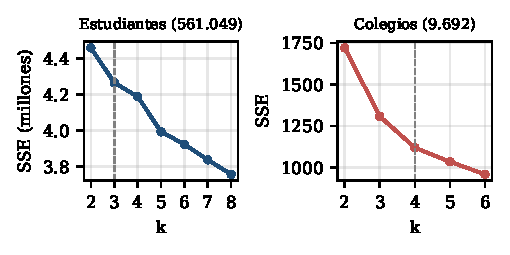
\includegraphics[width=\columnwidth]{fig/codo.pdf}
\caption{SSE intra-grupo de K-means en Weka para estudiantes y colegios.}
\label{fig:codo}
\end{figure}

\subsection{Resultados: estudiantes}
La SSE baja de 4.460.743 ($k=2$) a 4.267.542 ($k=3$) y a 4.189.772 ($k=4$), sin un codo claro (Fig.~\ref{fig:codo}). Con $k=3$, la corrida con semilla 42 da estos perfiles, que son ilustrativos y no robustos: un grupo de \emph{colegio privado acomodado} (20,8\,\%; 93\,\% con computador, 52\,\% con madre profesional; 291,3 puntos y 73,9\,\% en Alto), un grupo \emph{oficial con menos recursos y mayoría de mujeres} (58,9\,\%; 28\,\% con computador, 61\,\% con 10 libros o menos; 245,2 puntos y 40,7\,\% en Alto) y un grupo \emph{oficial, mayoría hombres} (20,3\,\%; 72\,\% con computador; 258,7 puntos y 51,8\,\% en Alto). Con $k=2$, \emph{classes to clusters} asigna mal al 39,1\,\% (en 2022, 47,2\,\%).

Sin embargo, estos grupos \textbf{no son estables}: el ARI entre la semilla 42 y las semillas 1 y 7 es 0,17 y 0,02. Con decenas de atributos nominales y distancia por coincidencias hay muchas particiones casi igual de buenas. Lo que sí se repite es un grupo con más recursos y mejor puntaje; la división del resto (incluido el corte por \texttt{estu\_genero}, que también apareció en 2022) depende de la inicialización. Por eso los perfiles anteriores describen una sola corrida y la conclusión útil sale del nivel colegio.

\subsection{Resultados: colegios (cruce con IPM)}
En colegios el codo es claro en $k=4$ (SSE para $k=2$, 3, 4 y 5: 1.719,7; 1.306,8; 1.118,9; 1.034,1). La Tabla~\ref{tab:colegios} y la Fig.~\ref{fig:colegios} muestran los cuatro tipos, ordenados por su puntaje medio, que K-means no vio:
\begin{itemize}
\item \textbf{C1 rural pobre} (2.237 colegios): 68\,\% rurales, en municipios con IPM medio de 51,6; 20\,\% con computador y 57\,\% de estudiantes que trabajan. 225,0 puntos.
\item \textbf{C2 oficial intermedio} (3.294): IPM 29,0, 37\,\% con computador. 243,2 puntos.
\item \textbf{C3 urbano conectado} (2.618): IPM 15,8, 67\,\% con computador, 54,4\,\% oficiales y 45,6\,\% privados. 265,5 puntos.
\item \textbf{C4 privado acomodado} (1.543): 95\,\% privados, 92\,\% con computador, 61\,\% de madres profesionales. 310,4 puntos.
\end{itemize}
Entre C1 y C4 hay \textbf{85 puntos}. Una regresión lineal del puntaje medio sobre los siete indicadores explica el 66\,\% de la varianza entre colegios ($R^2=0{,}659$), mucho más de lo que el perfil explica entre estudiantes. Aun así, entre el 10\,\% de colegios que más superan lo esperado por su contexto, el 65,1\,\% son oficiales, igual que su proporción total (65,4\,\%): rendir por encima del contexto no es exclusivo de los privados.

\begin{table}[t]
\caption{Tipos de colegio (K-means, $k=4$, 9.692 colegios)}
\label{tab:colegios}
\centering\small\setlength{\tabcolsep}{3.5pt}
\begin{tabular}{lrrrr}
\toprule
 & C1 & C2 & C3 & C4 \\
\midrule
Colegios & 2.237 & 3.294 & 2.618 & 1.543 \\
Estudiantes$^{*}$ & 83.677 & 205.266 & 193.234 & 71.598 \\
Puntaje medio & 225,0 & 243,2 & 265,5 & 310,4 \\
IPM del municipio & 51,6 & 29,0 & 15,8 & 14,8 \\
\% con computador & 20 & 37 & 67 & 92 \\
\% madre profesional & 5 & 9 & 19 & 61 \\
\% estudiantes que trabajan & 57 & 50 & 39 & 23 \\
\% privados / rurales & 4 / 68 & 18 / 29 & 46 / 8 & 95 / 11 \\
\bottomrule
\end{tabular}\\[2pt]
\parbox{0.95\columnwidth}{\footnotesize $^{*}$Suman 553.775 de los 561.049 estudiantes. Faltan 7.274: 7.175 en colegios con menos de 10 evaluados y 99 en 3 colegios sin IPM.}
\end{table}

\begin{figure}[t]
\centering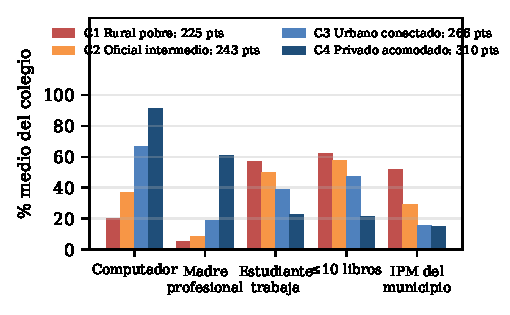
\includegraphics[width=\columnwidth]{fig/colegios.pdf}
\caption{Indicadores medios de los cuatro tipos de colegio y su puntaje.}
\label{fig:colegios}
\end{figure}

\section{Técnica 2: clasificación con árbol de decisión J48}
\subsection{Método}
J48 es la implementación de C4.5 en Weka: en cada nodo elige el atributo con mayor razón de ganancia y poda con un factor de confianza (0,25)~\cite{quinlan}. Entrenamos un árbol compacto ($M=1000$ instancias mínimas por hoja) y uno más detallado ($M=100$), con validación cruzada estratificada de 10 particiones (semilla 42) contra ZeroR. Para medir el aporte de los datos nuevos repetimos el árbol $M=100$ con tres conjuntos de atributos usando \texttt{FilteredClassifier}: los 18 de 2022, los 45 del ICFES sin cruces y los 48 con cruces. También calculamos la ganancia de información de cada atributo.

\subsection{Resultados}
\begin{table}[t]
\caption{Clasificación Alto/Bajo 2025, validación cruzada de 10 particiones}
\label{tab:j48}
\centering\small\setlength{\tabcolsep}{4pt}
\begin{tabular}{lrrrr}
\toprule
Modelo & Exactitud & Kappa & AUC & Hojas \\
\midrule
ZeroR & 50,15\,\% & 0,000 & 0,500 & -- \\
J48 $M$=100, 18 atrib. (2022) & 68,74\,\% & 0,375 & 0,747 & 1.595 \\
J48 $M$=100, 45 atrib. ICFES & 70,45\,\% & 0,409 & 0,765 & 1.550 \\
J48 $M$=100, 48 con cruces & \textbf{70,71\,\%} & \textbf{0,414} & \textbf{0,769} & 1.831 \\
J48 $M$=1000, 48 con cruces & 69,79\,\% & 0,396 & 0,759 & 248 \\
\bottomrule
\end{tabular}
\end{table}

Todos los árboles superan ampliamente a ZeroR (Tabla~\ref{tab:j48}). Con las mismas 18 variables de 2022, 2025 da 68,7\,\% con $M=100$; en 2022 se obtuvo 68,2\,\% con $M=1000$ y el mejor resultado fue 69,2\,\% con $M=2$. Los $M$ difieren, pero comparando el mejor árbol de cada año (69,2\,\% frente a 70,7\,\%) la relación entre perfil y puntaje es igual de fuerte. Las variables nuevas del ICFES suben 1,7 puntos y los cruces 0,3 más. El árbol de 248 hojas pierde menos de un punto y es más fácil de inspeccionar, aunque sigue siendo grande para leerlo completo.

\begin{figure}[t]
\centering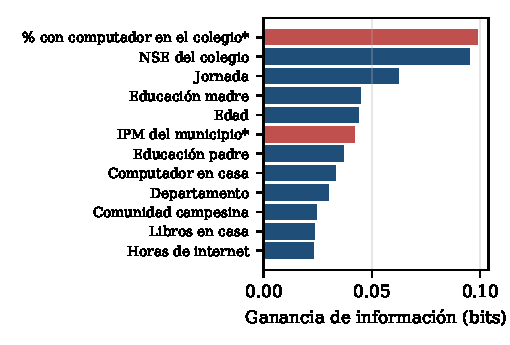
\includegraphics[width=\columnwidth]{fig/infogain.pdf}
\caption{Los 12 atributos con mayor ganancia de información (Weka). En rojo, los que vienen de los cruces.}
\label{fig:ig}
\end{figure}

\textbf{El colegio primero.} La raíz del árbol es el \emph{nivel socioeconómico del colegio} (NSE, calculado por el ICFES), y los dos atributos más informativos son de nivel colegio: el porcentaje de compañeros con computador (cruce, 0,099 bits) y el NSE del colegio (0,095), seguidos de la jornada (0,062), la educación de la madre (0,045), la edad (0,044) y el IPM del municipio (cruce, 0,042) (Fig.~\ref{fig:ig}). Tener computador en la propia casa aparece octavo (0,033) y el estrato del hogar apenas en el puesto 23 (0,012). Algunas reglas del árbol entrenado con todos los datos (los casos y el acierto son sobre el entrenamiento, no de validación cruzada; las reglas con 39.226 y 8.133 casos agregan varias hojas, no son hojas únicas):
\begin{itemize}
\item Colegio NSE4 $\Rightarrow$ Alto (35.957 casos, 92\,\% de acierto).
\item Colegio NSE1 $\Rightarrow$ Bajo (13.606, 76\,\%).
\item Colegio NSE2 y más de 20 años $\Rightarrow$ Bajo (10.389, 91\,\%); NSE2 y 18 años $\Rightarrow$ Bajo (39.226, 76\,\%).
\item Colegio NSE3, 17 años, 70--90\,\% de compañeros con computador y 11 a 25 libros en casa $\Rightarrow$ Alto (8.133, 68\,\%).
\item Jornadas nocturna y sabatina $\Rightarrow$ Bajo en todas las ramas con casos.
\end{itemize}
En colegios NSE3 oficiales, entre estudiantes de 17 años, el árbol separa por hábito de lectura: quienes leen por gusto 30 minutos o más quedan en Alto y quienes leen menos o nada, en Bajo.

\textbf{Hogar frente a colegio.} La Fig.~\ref{fig:nse} cruza el estrato del hogar con el NSE del colegio. Dentro de un mismo estrato, el colegio cambia todo: un estudiante de estrato~1 obtiene 237 puntos en un colegio NSE1 y 328 en uno NSE4 (91 puntos más). En colegios NSE4 todos los estratos obtienen entre 314 y 330. En colegios NSE1 y NSE2 la relación se invierte: el puntaje baja al subir el estrato del hogar (NSE1: de 237,0 en estrato~1 a 203,2 en estrato~6; NSE2: de 246,4 a 203,1), probablemente por selección de quiénes asisten a esos colegios. Las celdas de estratos 5 y 6 en colegios NSE1 son pequeñas (180 a 213 estudiantes) y deben leerse con cuidado.

\begin{figure}[t]
\centering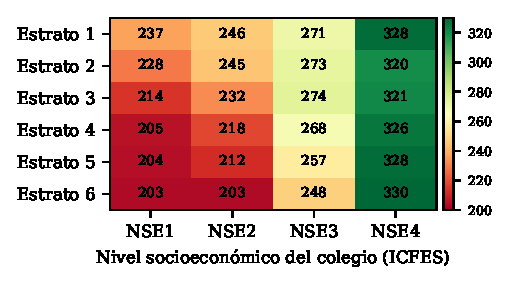
\includegraphics[width=\columnwidth]{fig/estrato_nse.pdf}
\caption{Puntaje global medio por estrato del hogar y nivel socioeconómico del colegio (561.049 estudiantes).}
\label{fig:nse}
\end{figure}

\textbf{Otras variables nuevas.} Estas brechas están en \texttt{results/2025/brechas.csv}~\cite{repo}. Los estudiantes que trabajan, aunque sea menos de 10 horas a la semana, obtienen 20,6 puntos menos que los que no trabajan (246,2 frente a 266,8); con más de 30 horas la brecha llega a 34 puntos. Tener más de 100 libros en casa se asocia con 42,2 puntos más que tener 10 o menos, y leer por gusto entre 30 y 60 minutos diarios, con 15,3 puntos más que no leer. Por municipio, el puntaje baja de 268,1 donde el IPM es menor a 20 a 223,8 donde supera 50, y la proporción en Alto cae de 58,3\,\% a 24,1\,\%.

\section{Técnica 3: refuerzo con bandit contextual}
\subsection{Planteamiento}
Weka no incluye aprendizaje por refuerzo, así que esta parte se hizo en Python. Un \emph{tutor virtual} atiende a los 561.049 estudiantes uno a uno y elige \emph{una} de cinco acciones: reforzar matemáticas, lectura, sociales, naturales o inglés. Es un \emph{bandit contextual}~\cite{li2010}, un problema de refuerzo de un paso donde el estado es el contexto~\cite{sutton}.
\begin{itemize}
\item \textbf{Contexto} $x$: 22 atributos en \emph{one-hot} más un sesgo ($d=110$): los 17 de perfil de 2022 más libros en casa, horas de trabajo, horas de lectura, NSE del colegio e IPM del municipio.
\item \textbf{Recompensa}: brecha estandarizada en el área elegida, $r_a=(\mu_a-y_a)/\sigma_a$. Es mayor cuanto más rezagado está el estudiante en esa área: mide el rezago, no el efecto de reforzarla.
\item \textbf{Retroalimentación parcial}: el agente solo ve la recompensa del área que eligió.
\end{itemize}
La acción óptima es el área más débil. Medimos el arrepentimiento acumulado $\sum_t(\max_a r_{t,a}-r_{t,a_t})$ y comparamos cinco políticas: aleatoria, siempre matemáticas, $\varepsilon$-greedy sin contexto y con contexto ($\varepsilon=0{,}05$), y LinUCB ($\alpha=0{,}5$), que elige $\arg\max_a\hat\theta_a^\top x+\alpha\sqrt{x^\top A_a^{-1}x}$ y actualiza $A_a^{-1}$ con Sherman-Morrison. Promediamos las semillas 1, 2 y 3; las políticas se evalúan \emph{in-sample}, sobre los mismos estudiantes con los que aprenden.

\subsection{Resultados}
\begin{table}[t]
\caption{Bandit contextual, 561.049 estudiantes (promedio de las semillas 1--3)}
\label{tab:bandit}
\centering\small\setlength{\tabcolsep}{4pt}
\begin{tabular}{lrrr}
\toprule
Política & Recomp. media & Arrepent. & Área óptima \\
\midrule
Aleatoria & 0,000 & 319.585 & 20,0\,\% \\
Siempre matemáticas & 0,000 & 319.522 & 20,8\,\% \\
$\varepsilon$-greedy sin contexto & 0,000 & 319.437 & 21,7\,\% \\
$\varepsilon$-greedy contextual & 0,080 & 274.493 & 25,9\,\% \\
LinUCB & \textbf{0,083} & \textbf{272.944} & \textbf{26,1\,\%} \\
Oráculo & 0,570 & 0 & 100\,\% \\
\bottomrule
\end{tabular}
\end{table}

Sin contexto no hay nada que aprender: las cinco áreas tienen recompensa media cercana a cero y $\varepsilon$-greedy sin contexto queda igual que el azar (Tabla~\ref{tab:bandit}). Con contexto, LinUCB reduce el arrepentimiento 14,6\,\% frente al azar y $\varepsilon$-greedy contextual 14,1\,\%; en 2022, con 17 atributos, la reducción fue de 12,3\,\%, así que las variables nuevas y el IPM ayudan también aquí (Fig.~\ref{fig:bandit}). La desviación estándar del arrepentimiento de LinUCB entre las tres semillas es 1.202.

La política aprendida es interpretable (perfiles promediados sobre las semillas 1--3, \emph{in-sample}). En colegios oficiales elige inglés el 44\,\% de las veces, en zona rural el 58\,\%, en municipios con IPM mayor a 50 el 55\,\% y en colegios NSE1 el 59\,\%. En colegios privados prefiere matemáticas (34\,\%) y lectura (23\,\%), y en colegios NSE4 lectura (58\,\%). Coincide con el área realmente más débil: inglés es la peor área del 28,1\,\% de los estudiantes de colegio oficial y del 28,4\,\% en municipios con IPM mayor a 50, mientras que en los privados la más frecuente es matemáticas (24,9\,\%). Aun así, la distancia al oráculo es grande (26,1\,\% frente a 100\,\% de aciertos), y el entorno es una simulación sobre datos fijos: la acción no cambia al estudiante. Como la recompensa mide el rezago, la política identifica el área más débil, pero no demuestra que reforzarla mejore el puntaje; eso exigiría medir el efecto causal de la intervención.

\begin{figure}[t]
\centering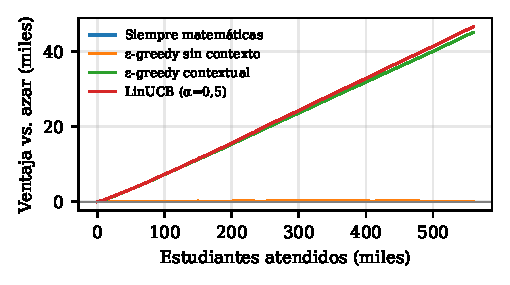
\includegraphics[width=\columnwidth]{fig/bandit.pdf}
\caption{Arrepentimiento evitado frente a la política aleatoria.}
\label{fig:bandit}
\end{figure}

\section{Comparación con 2022 y entre técnicas}
\begin{table}[t]
\caption{Saber 11 2022 frente a 2025 (brechas 2025 en \texttt{results/2025/brechas.csv})}
\label{tab:anios}
\centering\footnotesize\setlength{\tabcolsep}{3pt}
\begin{tabular}{lrr}
\toprule
 & 2022 (cal. A) & 2025 (ambos) \\
\midrule
Estudiantes analizados & 530.815 & 561.049 \\
Atributos / cruces & 18 / no & 48 / sí \\
Mediana del puntaje global & 247 & 254 \\
Brecha computador sí/no & 31,7 & 30,2 \\
Brecha privado/oficial & 28,8 & 27,7 \\
Brecha urbano/rural & 25,8 & 23,9 \\
Brecha hombres/mujeres & 7,3 & 8,9 \\
J48, 18 atributos & 68,2\,\% ($M$=1000) & 68,7\,\% ($M$=100) \\
J48, mejor & 69,2\,\% ($M$=2) & 70,7\,\% ($M$=100) \\
Mejor bandit vs. azar & $-$12,3\,\% & $-$14,6\,\% \\
\bottomrule
\end{tabular}
\end{table}

\textbf{Qué cambió frente a 2022 (Tabla~\ref{tab:anios}).} Las brechas son casi las mismas tres años después: unos 30 puntos por tener computador, 28 por estudiar en colegio privado y 24 por estudiar en zona urbana. La brecha por \texttt{estu\_genero} creció de 7,3 a 8,9 puntos a favor de los hombres; las cifras de 2025 se calcularon sobre los microdatos y están en \texttt{results/2025/brechas.csv}~\cite{repo}. Las medianas no son del todo comparables, porque 2025 incluye el calendario~B y el periodo 20251, cuyos 21.675 estudiantes promedian 282,4 puntos.

\textbf{Qué aporta cada técnica.} Las tres responden preguntas distintas con información distinta: K-means no usa el puntaje, J48 usa la etiqueta completa y el bandit solo ve la recompensa de lo que elige. Coinciden en lo esencial:
\begin{enumerate}
\item \textbf{El contexto del colegio pesa más que el del hogar.} El NSE del colegio es la raíz de J48 y los atributos más informativos son de nivel colegio; el agrupamiento de colegios explica el 66\,\% de su varianza, y dentro de un mismo estrato el colegio cambia el puntaje hasta en 91 puntos.
\item \textbf{La pobreza del territorio se suma.} El IPM del municipio está entre los seis atributos más informativos y separa al tipo de colegio con peor puntaje; el bandit, además, prioriza inglés donde el IPM es alto.
\item \textbf{El perfil no predice bien a cada persona.} J48 se queda en 70,7\,\%, los grupos de estudiantes son inestables y el bandit acierta el área óptima solo uno de cada cuatro (26,1\,\%) de los casos.
\end{enumerate}
En costo, cada corrida de K-means tomó unos 12~s, J48 con validación cruzada unos 2--3 minutos y el bandit unos 9 minutos para las 15 corridas.

\section{Conclusiones}
Con todos los resultados de Saber~11 de 2025 y dos cruces de bases, las tres técnicas muestran que el desempeño se asocia sobre todo con el contexto del colegio (su nivel socioeconómico y cuántos compañeros tienen computador), seguido de la jornada, la educación de la madre, la edad y la pobreza del municipio. Trabajar durante el bachillerato, tener pocos libros y no leer por gusto se asocian con puntajes más bajos. El árbol J48 alcanza 70,7\,\% de exactitud; los cruces y las variables nuevas mejoran dos puntos frente al modelo de 2022, pero no cambian el techo: la mayor parte de la diferencia individual queda sin explicar por variables de contexto. Las brechas casi no cambiaron entre 2022 y 2025. Todo lo anterior son asociaciones, no causas: el efecto del colegio mezcla la calidad de la enseñanza con quiénes asisten a él. Variables como estrato, etnia o \texttt{estu\_genero} deben usarse con cuidado para no estigmatizar. Como trabajo futuro, cuando los resultados de Saber Pro/TyT de esta cohorte estén disponibles y se obtenga acceso al catálogo longitudinal del ICFES, se podrá seguir a estos estudiantes (hoy Saber Pro solo está disponible hasta 2024); también se puede comparar con modelos como Random Forest.

\section*{Uso de inteligencia artificial}
En general, se usaron los agentes de IA Hark y Muse para apoyar el análisis y la redacción. Para el código (preprocesamiento, scripts de Weka, bandit y figuras) la IA usada fue Kiro CLI. Los autores revisaron los resultados, son responsables del contenido, y todos los integrantes entienden el trabajo.

\begin{thebibliography}{9}
\bibitem{dataicfes} ICFES, ``Bases y documentación técnica Saber 11°, microdatos 20251 y 20252,'' DataIcfes, 2026. [En línea]. Disponible: \url{https://www.icfes.gov.co/investigaciones/data-icfes/}
\bibitem{dane} DANE, ``Medida de pobreza multidimensional municipal de fuente censal 2018,'' 2020. [En línea]. Disponible: \url{https://www.dane.gov.co/index.php/estadisticas-por-tema/pobreza-y-condiciones-de-vida/pobreza-y-desigualdad/medida-de-pobreza-multidimensional-de-fuente-censal}. Boletín técnico: \url{https://www.dane.gov.co/files/investigaciones/condiciones_vida/pobreza/2018/informacion-censal/bt-censal-pobreza-municipal-2018.pdf}
\bibitem{weka} E. Frank, M. A. Hall e I. H. Witten, ``The WEKA Workbench,'' apéndice en \emph{Data Mining: Practical Machine Learning Tools and Techniques}, 4.ª ed. Morgan Kaufmann, 2016.
\bibitem{quinlan} J. R. Quinlan, \emph{C4.5: Programs for Machine Learning}. San Mateo, CA: Morgan Kaufmann, 1993.
\bibitem{li2010} L. Li, W. Chu, J. Langford y R. E. Schapire, ``A contextual-bandit approach to personalized news article recommendation,'' en \emph{Proc. WWW}, 2010, pp. 661--670.
\bibitem{sutton} R. S. Sutton y A. G. Barto, \emph{Reinforcement Learning: An Introduction}, 2.ª ed. MIT Press, 2018.
\bibitem{icfes22} ICFES, ``Resultados únicos Saber 11,'' Datos Abiertos Colombia, \texttt{kgxf-xxbe}. Disponible: \url{https://www.datos.gov.co/d/kgxf-xxbe}
\bibitem{repo} C. A. Lagos Malaver y L. G. Peraza Muñoz, ``saber11-aprendizaje-maquinal: código y resultados,'' GitHub, 2026. Los microdatos no se incluyen por su licencia de acceso restringido. [En línea]. Disponible: \url{https://github.com/its-camilo/saber11-aprendizaje-maquinal}
\end{thebibliography}

\end{document}
